We have discussed the problem statement and motivation in the previous chapter. In order to solve the problem stated in Chapter \ref{chap:1}, we have implemented a solution based on the machine learning approach. A clear understanding of concepts and terminologies of machine learning is required for the next chapters. Moreover, there are many different terms for a same concept in the areas of Data Science and Machine Learning which can be used interchangeably. Since later chapters will makes heavy use of these jargons it is necessary to establish a common base vocabulary to avoid confusion for the readers. So in this chapter we will explain Machine Learning and Scene Classification exhaustively. We will also discuss different computer vision tasks and how a neural network works.

% Image classification, Semantic Segmentation, Classification + localization, Object detection, , Instance segmentation.

% Machine learning and AI are frequently used as interchangeable terms. However, they are slightly different aspects of the same concept. In fact, AI is the parent to machine learning. https://towardsdatascience.com/artificial-intelligence-vs-machine-learning-a7d7a13b72d8


% In the previous chapter, we discussed the problem statement, motivation, and goals of this thesis. Again, in this thesis, we are trying to build an intelligent system that can classify the documents (tax-related) efficiently. I also mentioned that to solve this problem, we implemented different solutions but since our major solution is based on machine learning techniques, so we will mostly talk about that method. In the next few chapters, we will see and discuss the technologies and methodologies used to implement the solutions and how we trained a machine learning model for document classification but to understand these things, one need to have some pre-requisite knowledge in the domain of machine learning. So, in this chapter, we will explain the machine learning in detail. Along with that, we will also shed the light on core concepts of Artificial Neural Networks and Convolutional Neural Networks as it is a major part of the proposed solution.

\section{Artificial Intelligence and Machine Learning}
Artificial Intelligence and Machine Learning are often used together and in recent years has gained great popularity. Artificial Intelligence or AI is a broad area in Computer Science which mimics human intelligence. It focuses on theory and development of intelligent computer systems that can do activities like speech recognition, visual perception, decision-making, learning, planning, etc. AI systems need a large dataset to train its model and faster hardware to process the data. Artificial Intelligence has made significant advances in the past few years because of abundance of data through internet and cheap sensors and spectacular improvements in hardware capabilities.
\par
Machine learning is a specific subset of AI that trains a machine how to learn and improve from experience without being explicitly programmed. Machine learning is increasingly ubiquitous in consumer products such as smartphones, cheap sensors and IoT devices. Most of the people are using it in one way or another and without even knowing. Machine learning is changing our everyday life and powers so many aspects of our modern society. Some if it's applications are: search engine results refinement, spam/content filtering on social networks, Virtual Personal Assistants (like Siri, Alexa, Google Now), recommendations on e-commerce web-applications, online fraud detection, video surveillance, online customer support, and so on. There is a lot of research going on in this field. Researchers are proposing new applications of machine learning and also optimizing existing machine learning models.
\par
In machine learning, a model is trained by using some machine learning algorithms with a substantial amount of data to make predictions. There are a lot of different algorithms that work best for solving different problems, so we must have a good understanding of the algorithm to train our model before using it. Further sections aims to provide a rigourous, yet easy-to-follow, introduction of the main underlying concepts of machine learning, it's types and architecture.

% The recent era has witnessed many revolutionary wonders in the world of machine learning. By embracing the significance and power of it, the tech-communities around the globe are actively working on it and continuously striving to find the new horizons and possibilities in different domains to make things intelligent by leveraging the power of machine learning. According to the research, there are some tasks where machine learning has outperformed humans. The common applications of machine learning are mostly related to forecasting, classification, intelligent systems like voice assistants, etc. Furthermore, many commercial sectors are moving towards machine learning to automate their manual tasks and making their processes or systems intelligent. For example, banking sectors are using machine learning for fraud detection, in the health industry they are using it for disease diagnosis or forecasting, in online shopping portals, they are using it for showing items relevant to the user's interest. These are some of the few examples where different organizations are using machine learning to make their systems smart and independent and also to give users a better experience. 

% \par
% In machine learning, we train our model by using some machine learning algorithms with a huge amount of data to finally make predictions. There are a lot of algorithms that work best in different kinds of problems, so we need to have a better understanding of it before using any algorithm. Taking these things into account, further sections will explain the concepts of machine learning, it's types and architecture in detail.

\subsection{Definitions of Machine Learning}
A lot of scientists have given definitions of machine learning with respect to their own understanding and experiences. Below, it is presented some of the famous definitions of machine learning:
\newline
\newline
\par
\q{Machine learning research is part of research on artificial intelligence, seeking to provide knowledge to computers through data, observations and interacting with the world. That acquired knowledge allows computers to correctly generalize to new settings.} By Dr. Yoshua Bengio \cite{ml_def}
\newline
\newline
\par
Above is one of the definition of Machine Learning by Dr. Yoshua Bengio who also known as the godfather of Artificial Intelligence. Below are few more definitions from the well-known firms who are actively working on it.
\newline
\newline
\par
\q{Machine learning is based on algorithms that can learn from data without relying on rules-based programming.} By McKinsey \& Co. \cite{ml_def}
\newline
\newline
\par
\q{Machine Learning at its most basic is the practice of using algorithms to parse data, learn from it, and then make a determination or prediction about something in the world.} By Nvidia \cite{ml_def}
\newline
\newline
\par
\q{The field of Machine Learning seeks to answer the question “How can we build computer systems that automatically improve with experience, and what are the fundamental laws that govern all learning processes?} By Carnegie Mellon University \cite{ml_def}
% \subsection{History of Machine Learning}
\subsection{Evolution of Machine Learning}
Nowadays, if we look around ourselves, the power of machine learning has evolved to a point where it is mirroring the fictional tasks and enables the systems like self-driving cars, voice-activated assistants, smart appliances, etc but it didn't happen to occur in a few years but it has a long history of decades and tireless efforts of many scientists in this domain. In this section, we will try to give an overview of when and how this domain originated and how it got matured over the years.
\newline
\par
Before discussing the history, it should be noted that the core concepts of machine learning heavily rely on mathematics and statistics concepts. Many mathematical and statistical theories from the 18th century are the base of modern machine learning techniques of processing \cite{ml_history1} \cite{ml_history2} \cite{ml_history3}. These theories include the Least Squares method for data fitting by Adrien-Marie Legendre in 1805, Bayes' Theorem by Thomas Bayes and Pierre-Simon Laplace in 1812, etc. By taking theories as fundamentals, further work was done on machine learning. It all started in the 1950s in which many scientists developed different kinds of intelligent systems based on machine learning. 
\newline
\begin{itemize}
  \item \textbf{1950 - Turing Test:} The first intelligent program was the "Turing Test" designed by Alan Turing in 1950 \cite{ml_history1}. This program was designed to find out whether a computer will be able to think like humans or not. In this test, the human acted as an interviewer who asked questions to the system about a specific topic with a scenario. After that, the person has to tell whether the answers are given by the system or a human being. This test was meant to convince human beings that a computer can be capable of having human-level intelligence.
  \item  \textbf{1952 - Checkers Game:} In 1952, another intelligent system as the checker game was developed by Arthur Samuel \cite{ml_history2}. This game basically used to learn the checker's techniques and moves over the time and it got improved by playing more and more about which moves to lead to the winning and what can the bad move within a particular scenario.
  \item  \textbf{1957 — First Neural Network:} In 1957, Frank Rosenblatt designed PERCEPTRON, a single layer neural network model, which is considered to be the first neural network. It was designed to predict the pattern and shape recognition by mimicking the thought process of the human brain. Later on, in 1959, two other neural network models were created at Stanford University called ADALINE [REF] and MADALINE [REF]. ADALINE(Adaptive Linear Element) was able to recognize binary patterns from a stream of bits and can tell what can be the next bit while MADALINE (Many ADALINE) was able to remove the echo on phone lines.
  \item  \textbf{21st Century - The boom of Machine Learning:} Finally, the 21st century was the era when several tech giants have embraced the significance and power of machine learning and started to invest in this domain. Many neural networks were proposed by different scientists during a short period. Google Brain (2012), a deep neural network developed by Google primarily designed for pattern recognition. Another very famous and effective models were AlexNet(2012) \cite{1803.01164}, VGG16 and VGG19 \cite{vgg_19} (2014), ResNet (2015) \cite{1512.03385}, etc.
\end{itemize}
\subsection{Concept of Machine Learning}
In this section, we will explain the core concepts of machine learning also by emphasizing the above definitions. Machine Learning is a branch of Artificial Intelligence \cite{ai} which is used to make intelligent systems. As mentioned in the definitions, it uses different algorithms to learn from the huge amount of data to achieve a task and then make predictions or classifications based on the experience of training with given data without being explicitly programmed, unlike traditional programming. A few of the most common algorithms used by machine learning are Linear Regression, Naive Bayes, K-Nearest Neighbour (KNN), Support Vector Machine (SVM), etc. These algorithms work best in different scenarios like Naive Bayes works very good in text classification problems, support vector machines can be used for image classification, etc. One should have a little bit of understanding about these algorithms before choosing any algorithm for the problem. Each algorithm has its own way of learning from given data. In machine learning, we choose an algorithm to train a model to solve a particular problem, during training we pass a huge amount of data to the model so that it can learn from the data efficiently. For example, let say if the problem is related to the image classification or more specifically to classify different models of the vehicle then we have to pass the example data of these car models to our machine learning model. Here, I would like to mention that the model would only be able to classify those models whose data was present during the training. After training the model with this data, it will be able to classify the card models. The accuracy of its classification depends on the quality and quantity of data as it is directly proportional to the performance of prediction. So, how it is different from classical/traditional programming?
\begin{figure}[H]
\centering
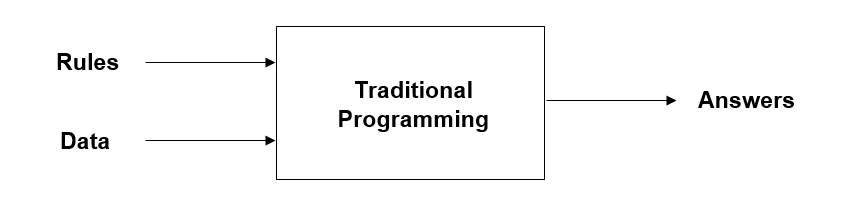
\includegraphics[scale=0.7]{images/Chapter2/TP.PNG}
\caption{Traditional Programming model}
\label{tp-model}
\end{figure}
\par
As you can see in the above Figure \ref{tp-model}, in traditional programming, there are two kinds of input required, first is the rules/logic and the second is data/input to the program and in the end, it will return the result as an answer. Basically, we have to implement the logic of the system and also specify the input data that the program expects. For example, if you want to create a program that should calculate employee's annual salary then you have to implement the entire logic of the program like from where the employee salary should fetch, what are the values that needs to be consider for calculation and also need to define the input parameters like employee id or name, year of salary calculation, etc. It means that this program is not independent and cannot run on its own unless these things have defined by someone.
\begin{figure}[H]
\centering
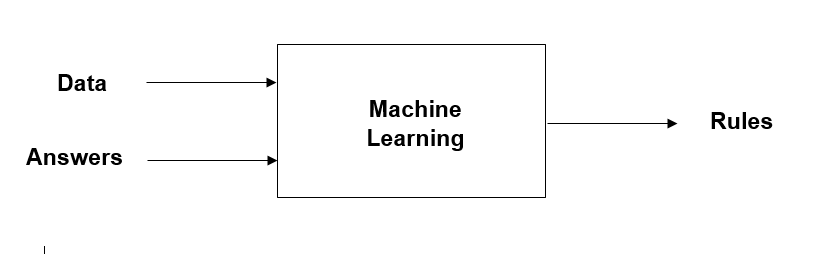
\includegraphics[scale=0.7]{images/Chapter2/ML.PNG}
\caption{Machine Learning model}
\label{mlp-model}
\end{figure}
\par
On the other hand, in machine learning, the inputs to the systems are data and answers and the result are rules. It means that to develop a machine learning program, we have to feed the program a lot of data as an input and at the same time we also have to tell the output or answers of these inputs. Based on these two things, the systems analyze the data and it's result and tries to learn automatically the rules to generate the result as output. Here, it should be noted that we are not implementing any kind of logic as we were doing in the traditional programming to generate the result explicitly but here the system learns or create that logic by itself which is actually the main feature of machine learning and in the end based on the learning from data and their answers, it will be able to perform further calculations or tasks by itself independently. We saw how machine learning is different and more powerful than traditional programming. We also tried to explain the basic concept behind machine learning which is that the dependency of the output heavily relies on the data and its output which we often call labels or tags in it.
\subsection{Training a model in Machine Learning}
Ever since the boom of machine learning has spread, many scientists have actively come forward and presented their model which was effective for different types of problems. However, the process of training a model has remained constant. In this section, we will give an insight view of how to train a machine learning model and what is the flow of training with the help of the below figure.
\begin{figure}[H]
\centering
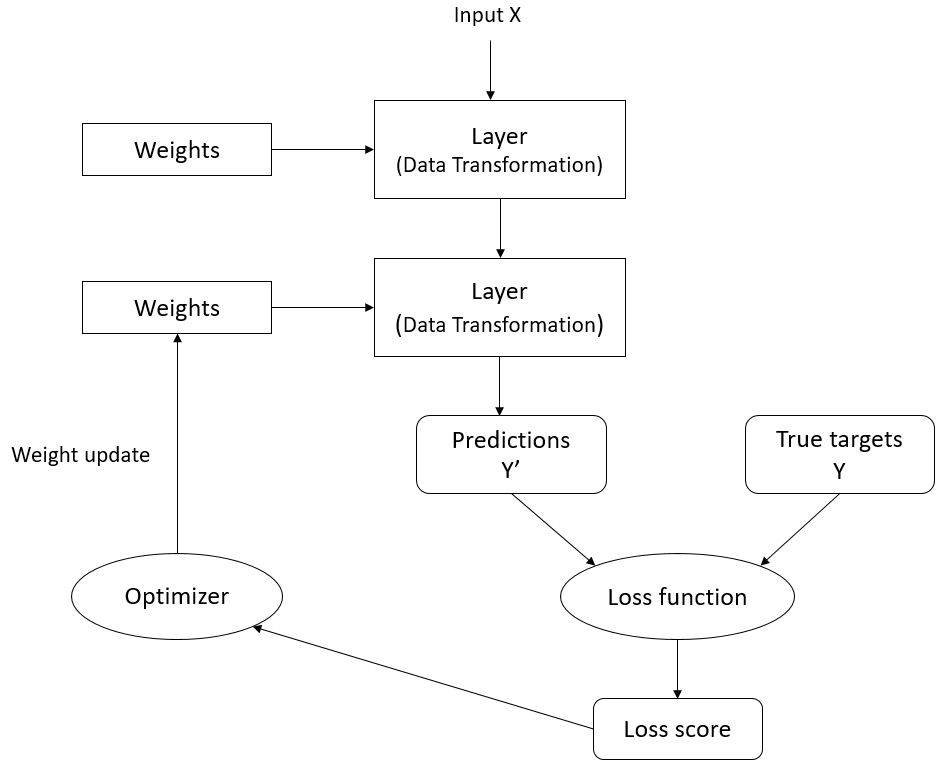
\includegraphics[scale=0.7]{images/Chapter2/ml-training-arch.png}
\caption{Machine Learning training architecture}
\label{mlt-arch}
\end{figure}
\par
Training a model consists of a complete cycle with different phases. Consider the above Figure \ref{mlt-arch} as a training architecture of a machine learning model. Let X is our training data for our model, the first step is to pass training data X to the Layers. Here, both the layers are considered as a machine learning model. In these layers, we can increase or decrease the layers of our model as per our requirement. In these layers, data is transformed into different forms. The purpose of this transformation is to make learning easier and efficient for our model. The technique for data transformation for the model varies with the different solutions as each one implements the solution according to their business model. Each layer in the model learns from the data and store particular information about it. During the training phase, the data passed to the model breaks into two parts, training and testing which is done to check the performance of the model. After processing all the input data by the model, now the prediction phase starts, and the model starts the prediction Y' on each input data. After all the predictions, the results Y' along with the true targets Y, which are the correct labeled pre-assigned to the data, passed to the loss function. In the \q{loss function}, we evaluate how well our training algorithm modeling the input dataset. If the predictions are not as expected, then it gives a higher number. If the predictions are good and as expected, then the output will be a smaller number. This output is in the form of a number and is called \q{loss value} which indicates whether our model is well trained for the given dataset or not. If the loss value is within the threshold then our model is fine and good to go but in case the loss value is very high, then there are some additional steps need to perform to minimize the loss value. In the case of higher loss values, we optimize or tune our weights for the model. Here, weights are the numerical value which are the parameters set for our model. The method of fine-tuning the weights are random and we need to keep hit and try until the satisfactory results are achieved. After optimizing weights, the same process starts again, to train the model with new weights on the given data X and then make predictions Y' and calculate the loss value with the help of loss function.
\subsection{Machine Learning Pipeline/Workflow}
In the previous section, we discussed the cycle of how to train a machine learning model. This section is kind of more generalize and here we will discuss that what is the starting point of the project, what are the essential phases involved to work on a full-fledged machine learning project, what is the sequence of these phases and the complete lifecycle this project. For this purpose and the sake of clarity, we will take the reference of the below figure to explain the whole process:
\begin{figure}[H]
\centering
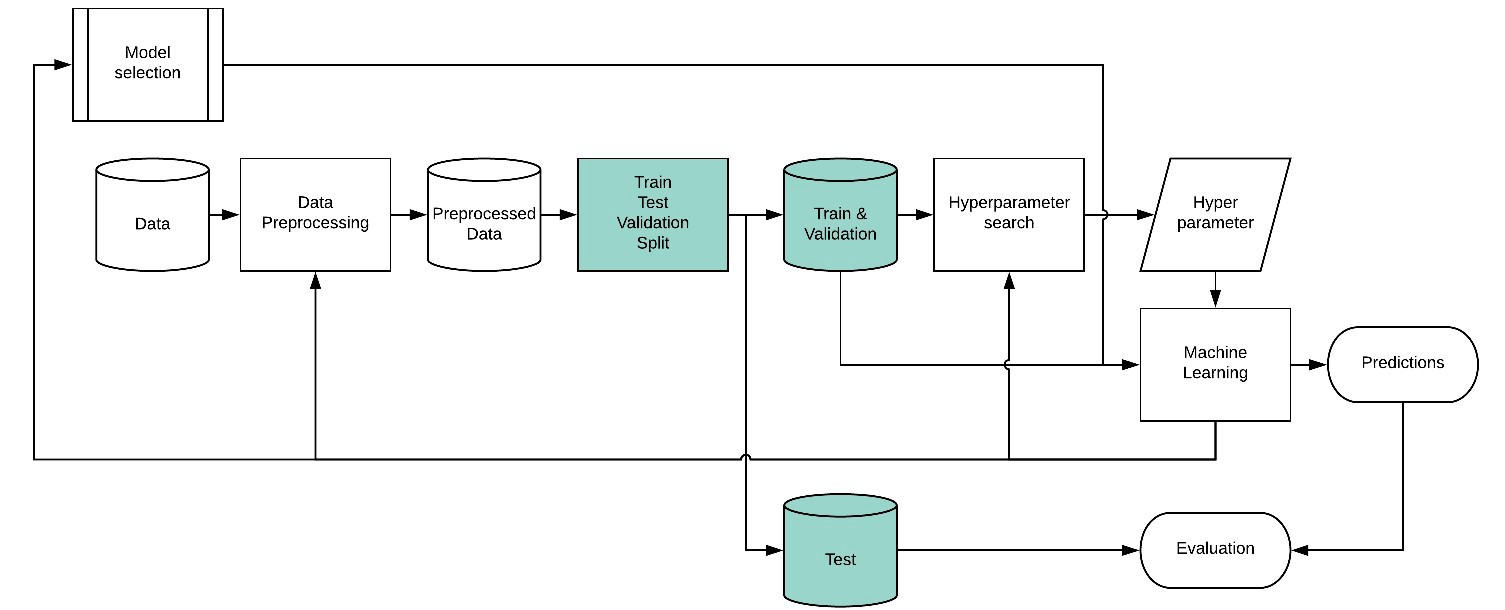
\includegraphics[scale=0.3]{images/Chapter2/ml-pipeline.jpg}
\caption{Machine Learning Pipeline design \cite{ml-pipeline}}
\label{ml-pipeline}
\end{figure}
\par
The above Figure \ref{ml-pipeline} represents a very comprehensive workflow of the phases/steps involved to build a machine learning application. Although the flow is pretty straightforward but there are few phases from where you can revert to the previous phase to modify or re-implement a process or parameter. Below are the major phases involved in the workflow.
\newline
\begin{enumerate}
  \item Data Gathering
  \item  Data Processing
  \item  Data Splitting
  \item  Model Selection
  \item  Model Training
  \item  Model Evaluation
  \item  Fine-Tuning Hyperparameters
  \item  Predictions
\end{enumerate}
\par
The most basic step to work on any kind of problem is to write \q{Problem description}. As soon as you have identified and analyzed the problem then you think about the possible solutions for the implementation. Likewise, also in machine learning, we are assuming that we have identified and wrote down the problem description and now the next step is to work on the data part and then later on implementation. Now let's try to simulate the solution with the above workflow. 
\newline
\par
As you can see in the above figure \ref{ml-pipeline}, the first few phases are related to data, which includes \q{data gathering}, \q{data pre-processing} and \q{splitting}. I have mentioned many times that the outcome or prediction of a machine learning model is heavily dependent on the data. So, the first phase towards the solution is to \q{gather the data} related to that problem and the data should be in high quantity. After data gathering, we can't directly use this data to train our model because this data is in raw format and cannot be understood directly by the computer, also it is fairly possible to have garbage data in the current dataset, therefore, the next phase is to clean the garbage or missing data so that our dataset contains only relevant data for our problem. Apart from data cleaning, we also convert raw data into a computer-readable format so that our model can learn efficiently from it. This step is called \q{Data Processing} or \q{Data Preparation}. Once we have cleaned and machine-readable data, we \q{split} the data into three parts which are train, test, and validation. The standard split ratio for train is 60\%, for test is 20\% and for validation is also 20\%. Here training data is used to train the model, validation data is used to fine-tune the parameters of the model to find out the accurate parameters and lastly, test data is used to evaluate the accuracy of the trained model.
\newline
\par
At \q{Model Selection} stage, data-related work is complete and now we have to select a model that best fits our problem. There are numerous models proposed by different scientists over the years and each model has its efficiency concerning the problem. Considering these things and our problem in mind, we select a model to further work with. After selecting a suitable model, the \q{model training} phase starts. In this phase, we train our selected model with processed data. Each model has its default hyperparameters, we can start training our model with default parameters and see how it goes. At the end of this phase, we will get a trained model that is ready for the prediction but first, we will test the performance and accuracy of prediction of our model by testing it with test data. Normally, we measure the performance by checking the loss value after training the model. This phase is called \q{Model Evaluation}.
\newline
\par
At the end of the model evaluation phase, there can be two scenarios, either the model is working fine which is quite ideal and unrealistic at the same time, in this case, our model is fine and good to go for future predictions. Another scenario is that our model is not predicting as expected and needs to be modified. From this stage, we can revert to multiple stages as if the results are totally off then maybe we are not using the suitable model and need to try other models. Other than that, if the results are a bit unexpected then we can tune the hyperparameter metrics and train our model again with new parameters or also check the data if there is any error or missing data and remove it. This phase is called \q{Fine-tuning Hyperparameters}. In this phase, we will keep hitting and try out these things until we have fine-tuned model which works well with all dataset. After getting the trained model, now we can use it to make \q{predictions} in our system with a different dataset.
\subsection{Terminologies used in Machine Learning}
\begin{itemize}
  \item \textbf{Loss Function:} 
  \par
  In the loss function, we evaluate how well our training algorithm modeling the input dataset.  If the predictions are not as expected, then it gives a higher number. If the predictions are good and as expected, then the output will be a smaller number. This output in the form of a number and is called loss value which indicates whether our training model is well trained for the given dataset or not.  If the loss value is within the threshold then our model is fine and good to go but in case the loss value is very high, then there are some additional steps need to perform to minimize the loss value.  In the case of higher loss values, we optimize or tune our weights for the model. Here, weights are the numerical value which are the parameters set for our model.
  \newline
  \par
    Furthermore, loss function can be categorized into two general categories which are Regression losses and Classification losses. Here the idea of regression and classification is the same as in machine learning. Some of the common regression loss functions are \q{Mean Square Error}, \q{Mean Absolute Error}, \q{Mean Bias Error} while classification loss functions are \q{Multi-class SVM Loss} and \q{Cross-Entropy Loss}.
  \item  \textbf{Gradient Descent Function:}
  \par
  Gradient Descent \cite{gd} is an algorithm which helps in finding the best-fit parameters (also called coefficients) that minimize the loss value of our loss function in a very efficient way and also in less iteration. Let's understand this with the help of an example. Assume a plotted graph of the cost function in the form of a bowl shape. For now, the current coefficients of the cost function are any point on the graph and the bottom of the bowl is the point where coefficients are best. Now, we have to hit and try random values of coefficients to reach that point. As you can see, this process can be very time-consuming and needs to be handled efficiently. Here, we need an algorithm that can take us to that point in as fewer iterations as possible and that is what the job of Gradient Descent algorithm.
  \item  \textbf{Overfitting}
  \par
  Overfitting is one of the major issues that can determine either a failure or success of a machine learning program. It is a scenario where the value of cost/loss function is low, but our model doesn't generalize well for the dataset which means that it works well for the dataset which was presented during the training but not on the new dataset. It generally happens when we leave our model training for so long that it picks up those features which were negative and was not supposed to learn. So, when the model tries to work on new data, those negative learned features do not apply to the new dataset which ultimately leads to poor prediction.
  \item  \textbf{Underfitting}
  \par
  Underfitting is a scenario where the model did not learn enough or well from the training and hence resulting in poor performance on the training data as well as on the new data. It is a problem that occurs when we choose a classifier that is too simple for the problem and is not suitable enough to capture the useful patterns in the data. Sometimes it happens in the result of avoiding overfitting.
  \item  \textbf{Generalization}
  \par
  Generalization is a property that refers that model has learned very well from the dataset during training which means it does not only work well on the dataset provided during the training but also works well on the future data which were not present during the training. What happens most of the time during the model training is that our model works very well for the training data but when we try to use it in some application where it has to predict or work on a totally new dataset then it failed to work well which indicates that our model is not generalized and can work well on a very closed dataset so it is very important to check the generalization of our model after training by checking its performance on the new dataset as well. This is something that is very important to have and is the ultimate goal for any machine learning project. Any model that doesn't generalizes the dataset considered to be either overfit or underfit.
\end{itemize}
\subsection{Types of Machine Learning}
So far, we have discussed the machine learning and how does it work in detail and now it's time to drill down further and discuss its types. Depending on the nature of problem, objective and algorithm, machine learning is categorized into three major categories
\begin{enumerate}
    \item \textbf{Supervised Learning}
    \item \textbf{Unsupervised Learning}
    \item \textbf{Reinforcement Learning}
\end{enumerate}
\subsubsection{Supervised Learning}
\par
Supervised learning is a methodology in which the program learns about a particular thing from its labeled examples or datasets to predict that thing in the future. Here labeled examples mean all the datasets will be labeled with correct answers and will be passed to the program to learn from it and remember the answer. It's just like teaching a child who doesn't know about a particular thing and we will give him/her different examples of it so that the child will understand that thing and can recognize it in the future. In supervised learning, our program analyzes the labeled datasets, store particular features from it and develop the rules to predict any future data. Below Figure \ref{ex-sl} is an example to demonstrate the idea of supervised learning
\begin{figure}[H]
\centering
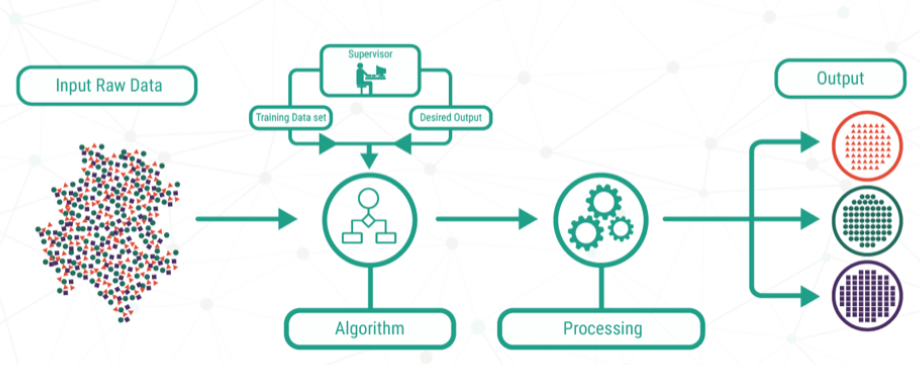
\includegraphics[scale=0.8]{images/Chapter2/supervised-learning-2.PNG}
\caption{Example of Supervised Learning \cite{sup_unsup_learning}}
\label{ex-sl}
\end{figure}
\par
For example, there is a system that has to detect whether an email is a spam or not. We have two categories for the classification: "Spam" and "Not-spam". Classification can be multiple as well. So, in the beginning, we are feeding the examples of both spam emails and not-spam(normal) emails to our model. The given examples or dataset to the system are properly labeled with its right class. Here, it is important to note that we have to feed the system enough examples in different formats or templates so that it can generalize the data well. After passing the data to the system, it processes the input and stores the rules and features for each classification class. After the model training, it will return the system which can predict future emails as spam or not spam. This thesis problem also aims to use supervised learning methodology to classify the tax-related document. 
\newline
\newline
Furthermore, supervised learning is further classified into two categories which are \textbf{Regression} and \textbf{Classification}
\begin{enumerate}[label=(\alph*)]
    \item \textbf{Regression:}
    \par
    In supervised learning, regression algorithms are used to estimate a mapping function (f) from the input variable (x) to continuous output variables (y). In simpler words, the output will always be in the form of continuous values means numbers. This continuous value can be either integer or float. It is mostly used to predict the amount or quantity. For example, by providing the KPIs of a company for the past 20 years we can use a regression algorithm to predict the KPI for next year.
    \item \textbf{Classification:}
    \par
    On the other hand, classification is used to predict or map the category of the given input instead of a value. The result of the classification algorithm will always be in the form of a discrete value. We normally use this methodology to assign classes to the given datasets. Since our thesis problem is related to the classification problem, we can take our problem to give an example. For example, given multiple tax-related documents to the classification algorithm, it will classify or predict the class/type of the document for the given dataset. Classification also has multiple types. For instance, if the classification is being done for only two classes then it is called \textbf{Binary Classification}. However, if we are dealing with more than two classes and the model has to predict a single class for a dataset from multiple classes then this problem is called \textbf{Multi-class} classification. Another type is where the model has to predict data into multiple classes with percentage then this is called \textbf{Multi-Label Multi-class} Classification.
\end{enumerate}
\subsubsection{Unsupervised Learning}
\par
In unsupervised learning, as the name suggests there is no supervision or help provided about the dataset to the model. In this scenario, we do not know the result of the prediction or classification. Here, we pass plain and unstructured data to the model and now it's the job of the model to detect and recognize the pattern from the dataset and learn from it. It is normally used to extract the insights from the unstructured data and to cluster the data into multiple groups without knowing the actual categories.
\begin{figure}[H]
\centering
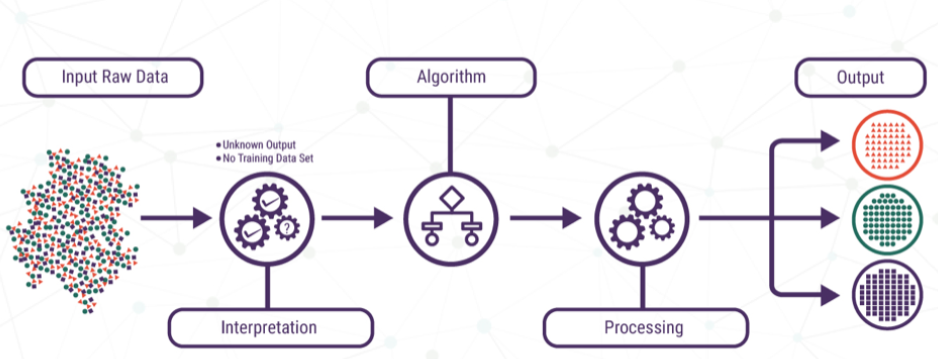
\includegraphics[scale=0.7]{images/Chapter2/unsupervised-learning.PNG}
\caption{Example of Unsupervised Learning \cite{sup_unsup_learning}}
\label{ex-ul}
\end{figure}
\par
As you can see in the Figure \ref{ex-ul}, we are providing raw data to the model which means there is no label attached to the dataset, it is a totally new dataset for the model, and it does not have any knowledge about the types. Here what will the model do is to start looking for the pattern in the dataset. For instance, if the dataset is in the form of text and the model is getting particular keywords in some of the data every time then it will cluster these datasets into a different group and at the end, it will cluster all the data into different groups based on its finding.
\subsubsection{Reinforcement Learning}
\par
Reinforcement learning is a methodology where the model learns over time by interacting with the environment. We can consider it as an intelligent system that learns from its experiences. For example, if the system is exposed to an environment and it has to predict the class of an image, it may happen that it will predict the wrong class but what will happen at that point is that someone will correct the system and tell the model about the correct class. Here, the model will update its information and will try to predict it correctly next time based on its previous experience. So, in reinforcement learning, the model is in continuous contact with the agents who correct the system about the wrong prediction and ultimately it will get mature by time and start predicting correctly.
\begin{figure}[H]
\centering
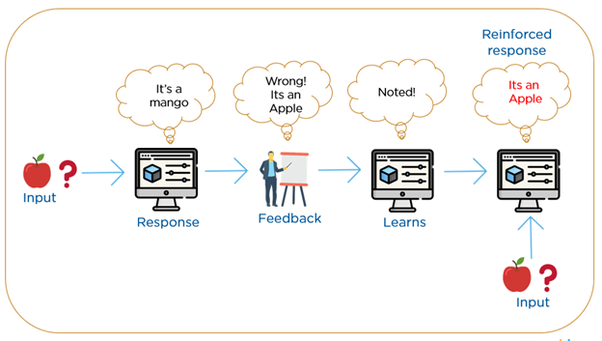
\includegraphics[scale=0.7]{images/Chapter2/reinforcement-learning.png}
\caption{Example of Reinforcement Learning \cite{rei_learning}}
\label{ex-rl}
\end{figure}
\section{Artificial Neural Network}
Historically, neural networks are responsible for the revival of interest in machine learning. The subject of Artificial Neural Network (ANN) has matured to a great extent over the past few years and especially with the advent of very high-performance computing, the subject has assumed a tremendous significance and has got a very big application potential in very recent years. It met a lot of success in practical applications and got people going. Furthermore, many organizations are using it as a standard for example in banking and credit approval, medicine study, disease diagnosis neural networks are often used.
\subsection{Definition and Description}
\q{Artificial Neural Network (ANN) is a computational model that takes the inspiration of how the human brain works and how it processes the information and tends to replicate it as a system. In this system, it learns to perform tasks by learning from past examples without being programmed.} \cite{ann_def}
\newline
\newline
\par
Artificial Neural Network also known as Neural Network is part of a broader family of machine learning. This computational model is used to make intelligent systems. ANN basically mimics the way the human brain works and is also built on the same pattern. For example, if we want to teach a program to do a specific task then what are the possibilities of teaching that we can think of? The very basic approach is to write the whole program in the form of instructions (programming code) where the program will follow the instructions and perform the task accordingly. This program is not intelligent and is totally dependent on the given instruction. On the other hand, we can let the program to learn on its own which means we can apply artificial intelligence in the form of neural networks. 
\par
As I mentioned earlier, neural networks are capable of performing a task the way human beings do but in case of human beings they are not explicitly programmed instead a human mind learns themselves from examples and experiences and next time when it has to perform the same task, it follows the previous learning from examples and performs the tasks. For instance, let's take the example of our thesis problem where we have to classify the tax-related documents. If we ask a human being to classify and recognize these tax documents, then how a human brain will perform it? Well, it depends, if there is a document that a human brain never saw or processed before then obviously it will not recognize it at first because there is no previous learning or example that exists related to this document. In this case, the human brain will store this experience. Obviously, one example is not sufficient to generate a concrete memory and the human brain has to go through several documents of the same type to finally generate reliable learning and memory. When the human brain was going through these documents, what happened is that it analyzes the document, detects the patterns or keywords. Let say, in case of a salary slip document, there are many keywords that are always present normally such as net income, gross income, income tax, insurance tax, etc. So, what human brain will do is to store these keywords or if the document pattern or structure is the same then it also stores it as a feature. Now, next time when it has to recognize the same document, it will look for the same keywords and patterns which it has seen in the previous examples and made a decision based on that whether a document is of which type. This is a small example of human brain capacity and methodology to perform any task.  In the same way, the neural network learns from the examples given to it, develop the rules by processing, extracting and storing the features in different ways and use this learning to perform future tasks related to it.

\subsection{Architecture of Neural Network}
The basic architecture of a neural network consists of three layers: input, hidden layer and output. However, these hidden layers can be increased as well within a neural network. Each layer consists of neurons that are fully connected with each other. These connections are responsible to transmit data from one neuron to another. Below Figure \ref{ann-archi} is an example of a basic neural network architecture.
\begin{figure}[H]
\centering
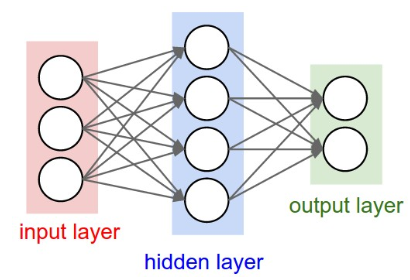
\includegraphics[scale=0.7]{images/Chapter2/ann-arch.PNG}
\caption{Architecture of Neural Network \cite{ann_arch}}
\label{ann-archi}
\end{figure}
\par
As we see that neural network built on a layered architecture and each layer consist of neurons and are responsible for a particular job. Here the input layer is responsible for receiving data from outside the network it means whenever we feed data to the neural network to learn something it first passed through the input layer. Some scientists have said that the neurons in the input layer are different from the neurons in the subsequent layers and they do not receive information from the previous layer. It also makes sense to an extent because this input layer is the entry point to the network and does not contain any previous layer. So, in simpler words, the input layer is only responsible to receive data from outside and pass it on to the subsequent layer which is a hidden layer to process the data. The hidden layer is found between the input and output layers. As I said, the hidden layer in neural networks contains a minimum of one layer and then the number of hidden layers can be increased or decreased based on the complexity of the problem. The primary role of is layer is to receive data from the input layer and do some processing on this data like feature extraction, storing the features in the form of edges, etc. and produce the output by an activation function for the next layer. In short, all the processes related to the learning of the neural network is performed in the layer. The output layer which is the final layer is responsible to receive the data from the hidden layer and ultimately produce the end-result for the neural network.
\subsection{In-depth detail of Artificial Neural Network}
In this section, we will dive deep into the world of neural networks and will see the internal processing of neural networks. In the previous section, we described the different layers involved in the network and what are the responsibilities of each layer. Each layer consists of interconnected neurons or also known as nodes. In artificial neural networks, artificial neurons built by taking inspiration from the biological neurons present in the human brain.
\begin{figure}[H]
\centering
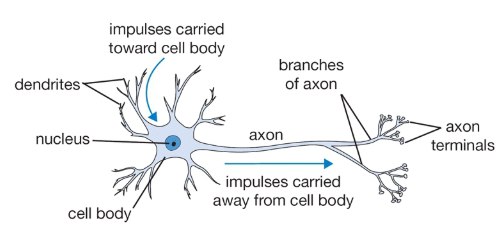
\includegraphics[scale=0.9]{images/Chapter2/neuron.PNG}
\caption{Illustration of Biological Neuron \cite{ann_arch}}
\label{neuron}
\end{figure}
\par
In a biological neuron, \q{Dendrites} are responsible to receive the chemical signals from other neurons then applies a summation function which is adding all the inputs multiplies by the weight associated with it and then the \q{Axon} receives the output of summation and then passed it to the other neurons as a signal. An artificial neuron, somewhat, behaves in the same way as the biological neuron does. Likewise, artificial neurons in the neural network are the most fundamental computational unit which takes input from the different neurons, then applies some function to generate an output which is later on passed to some other neuron. Each input received by the neuron has a weight "w" associated with it and in the function, we take the summation of input x multiplied by its weight to generate the output Y. Below is the picture representing the described process.
\begin{figure}[H]
\centering
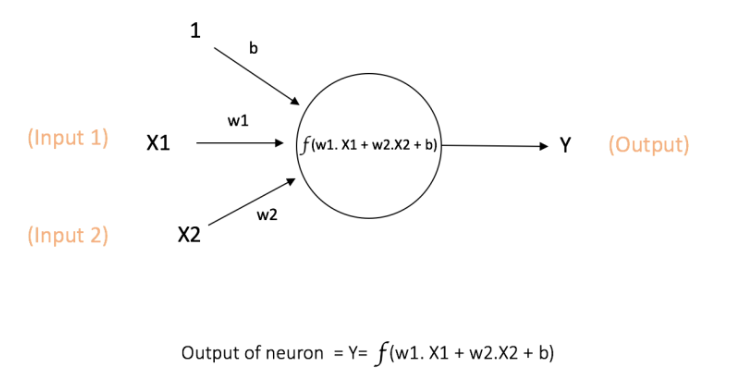
\includegraphics[scale=0.9]{images/Chapter2/neuron-summation-func.png}
\caption{Artificial Neuron \cite{intro_to_nn}}
\label{neuron-sum-func}
\end{figure}
\par
In general, whenever a neural network is used to solve a problem, we first train our neural network by feeding the data to it. This data entered through the input layers and then pass it on to the hidden layers which are basically responsible for analyzing the data learn from it. If the hidden layers are multiple then in each layer, it stores different types of information. The result of the hidden layer(s) is the final output which is passed on to the output layer and then can be consumed by the system. Let's understand it with the help of below example of how neural network learns from the data.
\begin{figure}[H]
\centering
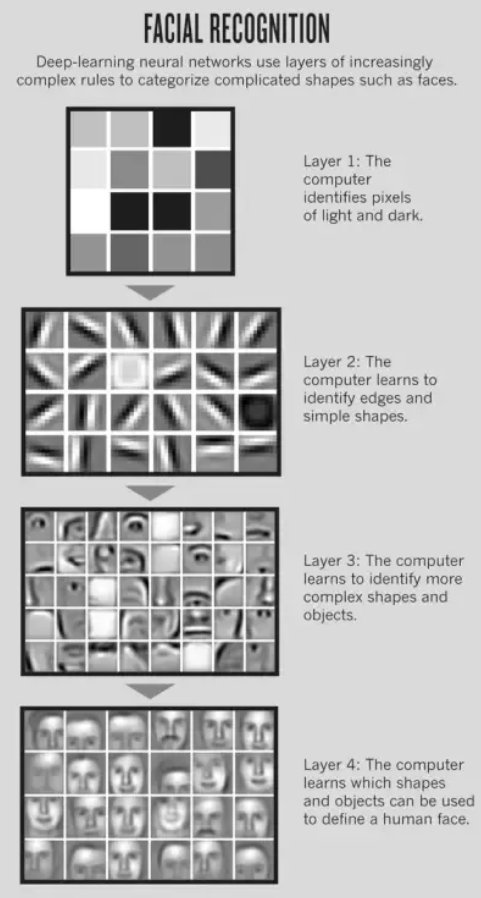
\includegraphics[scale=0.6]{images/Chapter2/ANN-example.PNG}
\caption{Facial recognition example of Neural Network \cite{hidden_layer}}
\label{fr-ex-neural-network}
\end{figure}
\par
In the above example, the task is to detect a human face with the help of a neural network. For this, they are using a neural network that consists of multiple hidden layers and in the above diagram, these layers can be considered as the hidden layers. As you can see, each layer is storing some kind of information that is used to identify any particular information and the complexity of information is increasing by each layer. The first layer is used to identify the pixels of data then in the second layer, it identifies the edges from the data by the help of information from the first layer. In the third layer, it broke down the information into different human face objects like nose, ears, eyes mouth, etc. and trying to identify them. By the fourth layer, the network can detect a human face.
\section{Convolutional Neural Network (CNN or ConvNet)}
Convolutional Neural Network (CNN) is a type of artificial neural network which consists of convolutional layers and has been very successful particularly related to computer vision tasks such as recognizing objects, scenes, faces, etc. among many other applications. We have probably seen them in action anywhere a computer is identifying objects in an image, but we can also use the convolutional neural network in natural language procession projects which are primarily used for text classification too. The fact that they are useful for these fast-growing areas is one of the reasons they are so important in deep learning and artificial intelligence domain today. Once we understand how CNN works and what makes it unique from other neural networks, we can see why they are so effective for processing and classifying images.
\newline
\par
But let's first take a regular neural network. A regular neural network has an input layer, hidden layers, and an output layer. The input layer accepts input in different forms while the hidden layers are responsible for performing calculations on these inputs and the output layer then delivers the outcome of the calculations and extractions. Each of these layers contains artificial neurons that are connected to neurons in the previous layer and each neuron has its own weight. This means we are not making any assumptions about the data being fed into the network. Usually, it works but not if you are working with images or a language. CNN works differently as they treat data as spatial. Instead of neurons being connected to every neuron in the previous layer, they are instead only connected to neurons close to it and all have the same weight. This simplification in the connection means the network upholds the spatial aspect of the dataset. The word convolutional refers to the filtering process that happens in this type of network. Think of it this way, an image is complex, and a convolutional neural network simplifies so it can better be processed and understood.
\subsection{Architecture of Convolutional Neural Network}
\begin{figure}[H]
\centering
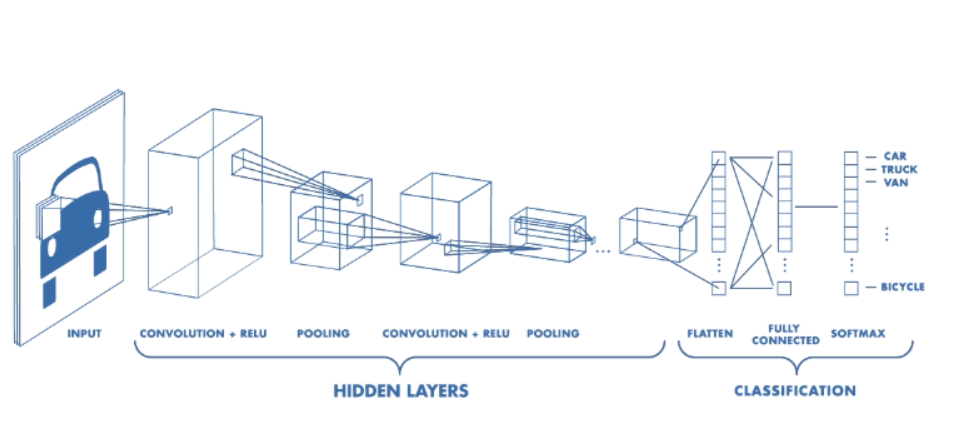
\includegraphics[scale=0.7]{images/Chapter2/cnn-arch.png}
\caption{Architecture of Convolutional Neural Network \cite{arch_cnn}}
\label{cnn-arch}
\end{figure}
\par
Let's look at what is inside a convolutional neural network architecture. Like a normal neural network, a CNN is made up of multiple layers. There are a couple of layers that make it unique which are the \q{convolutional layer} and the \q{pooling layer}. However, like other neural networks, it will also have an \q{activation function} and a fully connected layer. The activation function layer ensures the non-linearity as the data moves through each layer in the network. Without it, the data being fed into each layer would lose the dimensionality that we want to maintain. On the other hand, the fully connected layer meanwhile allows us to perform classification on the dataset. In this architecture, the convolutional layer is the most important layer. It works by placing a filter over an array of image pixels and this then creates what is called a convolved feature map. It's a bit like looking at an image through a window which allows you to see specific features you might not otherwise be able to see. Next, we have the pooling layer. Its firsts reduce the sample size of a particular feature map. This also makes processing much faster as it reduces the number of parameters the network needs to process. The output of this is a pooled feature map. There are two ways of doing this, \q{max pooling} which takes the maximum input of a particular convolved feature or \q{average pooling} which simply takes the average. These steps are used for feature extraction whereby the network builds up a picture of the image data. If we want to perform classification, you will need to move into the fully connected layer. To do this, we will need to \q{flatten} things out. Remember, a neural network with a more complex set of connections can only process linear data.
\newline
\par
Throughout the years, several scientists have worked and proposed different architectures of CNN. Few of them are \textbf{LeNet}(1990s), \textbf{AlexNet}(2012), \textbf{ZF Net}(2013), \textbf{GoogleNet}(2014), \textbf{VGGNet}(2014), \textbf{ResNet}(2015), etc. In this thesis, we have used the VGGNet architecture of CNN to classify the tax-related documents.
\subsection{Operations in Convolutional Neural Network}
There are couple of operations involved for different purposes within the convolutional neural network. Here, we will have a look on them one by one.
\subsubsection{Activation Function}
In CNN, the Activation function \cite{activation_func} is used to introduce non-linearity in the output of the neuron. When neuron generates the output by the weighted sum of inputs and adding bias then activation function is responsible to decide whether this output should be considered as fired neuron not to the other neurons. Some of the common activation functions are ReLU, Sigmoid, Softmax, tanh, etc.
\subsubsection{Convolution}
In a convolutional neural network architecture, we use a convolution operation in the convolutional layer. The main goal of the convolution operation is to maintain the spatial connection between pixels. It works by placing a filter over an array of image pixels and this then creates what is called a convolved feature map.
\subsubsection{Bath Normalization}
Batch normalization is the process of implementing normalization to the activation layer by subtracting the batch mean and dividing by the batch standard deviation. The main purpose of doing so it to faster the process of training within the convolutional neural network.
\subsubsection{Pooling}
The pooling operation is used to reduce the dimensionality of the feature maps, but it retains the most important information. The output of this operation is called Pooled Feature Map. There are two types of pooling, \textbf{max pooling} that takes the largest element from the feature map within a window and the \textbf{average pooling} which takes the average of all the elements within a window.
\subsubsection{Padding}
Padding operation is used to add more window to the image by adding extra pixels at the border of the image. It is used to retain a better understanding of the edges of the image by centralizing it. Some of the padding's operations are \textbf{zero padding} and \textbf{reflection padding}. 